\clearpage

\section{Theorie}
\label{theorie}

\subsection{Mobilfunkstandards}

\subsection{SIM-Karten}

\subsection{Authentifizierungsvorgang}
\label{authentifizierungsvorgang}

\subsection{Milenage Algorithmus}
\label{milenage}
Zwischen \ac{SIM}-Karte und Netzprovider muss eine sichere Authentifizierung und Kommunikation gewährleistet werden können. Dies war wie in Kapitel \ref{geschichte-usim} bereits beschrieben mit dem ersten entwickelten Algorithmus des \ac{3GPP} nicht mehr gewährleistet, weshalb mit der Entwicklung des neuen Netzstandards auch ein neuer Algorithmus entwickelt wurde, namentlich der Milenage Algorithmus. \\
Dieser verfügt über die sieben Funktionen \emph{f1}, \emph{f1*}, \emph{f2}, \emph{f3}, \emph{f4}, \emph{f5}, \emph{f5*} mit Hilfe derer eine sichere Authentifizierung und Schlüsselgenerierung ermöglicht wird. 3GPP hat allerdings wie auch beim Vorgänger diese Funktionen nicht näher spezifiziert und ermöglicht den Netzprovidern eigenen Lösungen zu implementieren. Stattdessen beschrieben sie den Kontext in dem diese Funktionen Anwendung finden und definieren generelle Anforderungen an diese Algorithmen \cite{3gpp.35.205}.

Der Milenage Algorithmus hat wie erwähnt zwei Hauptaufgaben, nämlich einerseits die Authentifizierung, als auch die Generierung eines Schlüssel, um die versendeten Nachrichten zu ver- und entschlüsseln. Wenn es um die Authentifizierung geht muss sich einerseits die SIM-Karte, bzw. das \ac{UE}, gegenüber dem Netzprovider authentifizieren, aber andererseits muss sich auch das Netzwerk gegenüber der SIM-Karte authentifizieren. Damit soll die Möglichkeit der Man-in-the-Middle Attacken reduziert werden, die es einem Außenstehenden erlauben die Kommunikation mitzulesen. Auch so genannte Replay-Attacken, bei denen zuvor aufgezeichnete Daten genutzt werden, sind nicht möglich, auf Grund der \acl{SQN} \cite{spitz11}.

In den nachfolgenden Unterkapiteln wird die Funktionsweise des Algorithmus, sowie die Funktionsweise der eingesetzten Blockschiffrierung \ac{AES} erläutert.

 \subsubsection{Funktionsweise}
 In Kapitel \ref{authentifizierungsvorgang} wurde beschrieben, welche Daten zwischen \ac{AuC} und \ac{UE} verschickt werden, jedoch nicht wie diese Daten generiert werden. Es gibt einige Werte, die auf der \ac{USIM} und der Datenbank des \ac{AuC} fest eingespeichert sind. Diese sind der \ac{OP} und \ac{K}, sowie jeweils fünf Rotations- und XOR-Konstanten (r1, ..., r5 und c1, ... c5). Welche Funktion welche Werte benötigt und generiert zeigt dabei Abbildung \ref{abb:funktionsubersicht}.
 
 \begin{figure}[htp]
  \begin{center}
   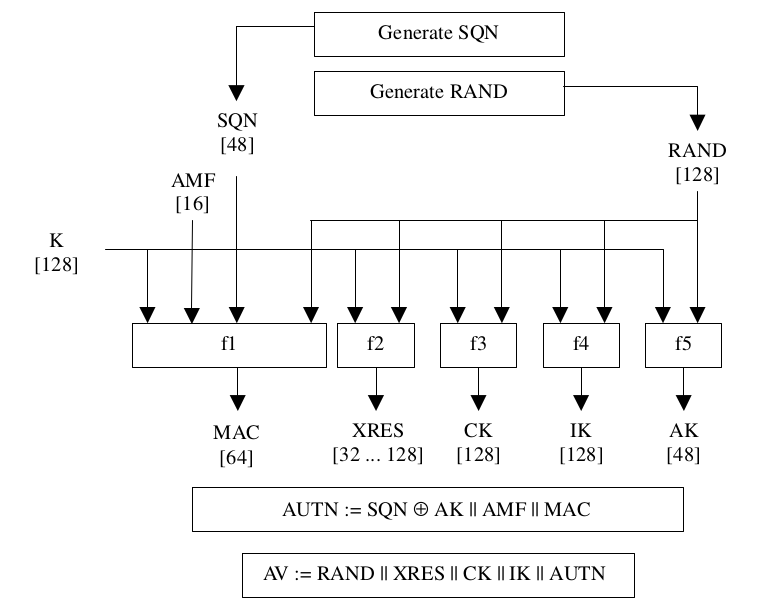
\includegraphics[width=300pt]{generation_of_authentication_vectors}
  \end{center}
  \caption{Übersicht über die Generierung der Authentifizierungsvektoren \cite{3gpp.33.102}}
  \label{abb:funktionsubersicht}
 \end{figure}
 
 In Abbildung \ref{abb:funktionsubersicht} ist zu sehen, dass zu Beginn die \ac{SQN} generiert wird. Diese ist insgesamt 48 Bits lang und besteht aus den beiden Teilen SEQ und IND, mit SEQ als der die eigentliche Sequenznummer und IND als Arrayindex. Dieser Index wird benötigt, da auf der SIM-Karte sind die letzten SQNs in einem Array gespeichert. Die empfohlene Arraygröße ist 32, was für IND eine Länge von fünf Bits bedeutet. Mit diesem Index kann nachher die Aktualität der SEQ überprüft werden.\cite{3gpp.33.102} \\
 Für die Bildung der SEQ selbst gibt es drei verschiedene Möglichkeiten:
 \begin{itemize}
  \item teilweise zeitbasiert
  \item nicht zeitbasiert
  \item komplett zeitbasiert
 \end{itemize}
 
 Die einfachste Variante ist die nicht zeitbasierte Lösung, bei der lediglich ein Zähler hochgezählt wird mit jeder Authentifizierungsanfrage. Die SEQ ist initial also 0 und wird hochgezählt und gleichzeitig vom \ac{AuC} in einer Datenbank gespeichert \cite{3gpp.33.102}. Auf die anderen Möglichkeiten wird hier nicht näher eingegangen, da sie in dieser Arbeit keine Anwendung fanden.
 
 Als nächstes wird die \ac{RAND} gebildet. Das Verfahren, wie der Netzprovider diese RAND generiert darf nicht offen gelegt werden, da dies die Sicherheit stark beeinflussen würde. Generell handelt es sich dabei um eine 128-bit lange Zufallszahl, die für jede Funktion benötigt wird.
 
 Abbildung \ref{abb:funktionsubersicht} zeigt zwar, welche Variablen in die Funktionen einfließen und welche Werte sie zurückgeben, aber sie zeigt nicht näher wie diese Werte nun verarbeitet werden. Dies zeigt Abbildung \ref{abb:schematisch_milenage} besser. Dort ist zu erkennen, dass \emph{f2} bis \emph{f5*} nach dem selben Schema berechnet werden können und \emph{f1}, sowie \emph{f1*} noch einige zusätzliche Parameter haben.
 
 Zunächst die Erklärung der Symbole sowie einiger weiterer Abkürzungen. \ac{OPc} wird durch folgende Formel generiert:
 \begin{center}
  $OP_{C} = OP \oplus E(OP)_{K}$
 \end{center}
 
 $E()$ ist die Blockschiffrierung. In diesem Falle wird also \ac{OP} mit dem Schlüssel \ac{K} verschlüsselt. Welche Verschlüsselung gewählt wird, wird von 3GPP nicht vorgegeben. In dieser Arbeit wurde \ac{AES} verwendet, welche im Kapitel \ref{aes} näher beschrieben wird. \\
 Der verschlüsselte OP wird dann im zweiten Schritt über XOR ($\oplus$) mit dem ursprünglichen OP verknüpft.
 
 \begin{figure}[ht]
  \begin{center}
   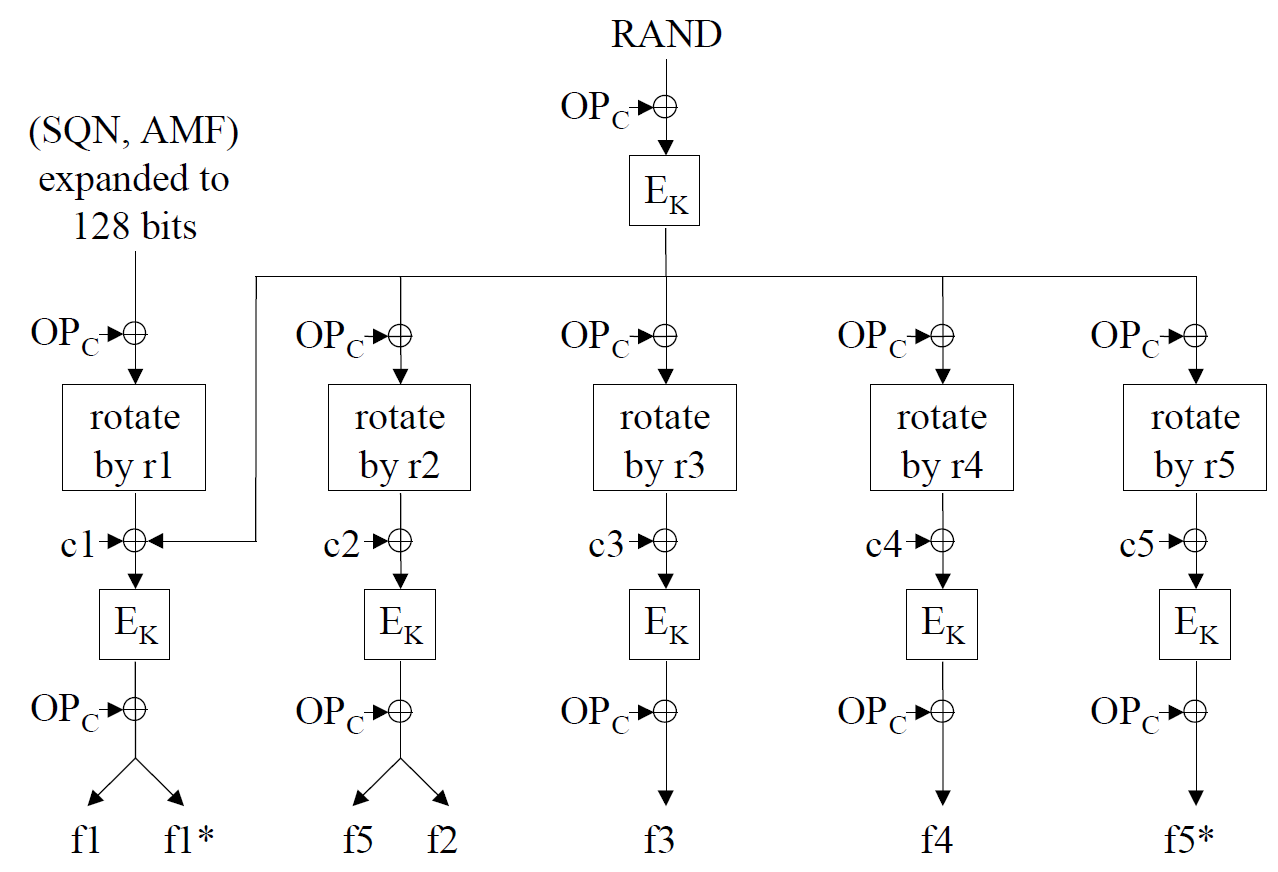
\includegraphics[width=400pt]{detailed_generation_of_authentication_vectors}
  \end{center}
  \caption{Schematische Darstellung zur Berechnung der Authentifizierungsvektoren \cite{3gpp.33.102}}
  \label{abb:schematisch_milenage}
 \end{figure}
 
 In Abbildung \ref{abb:schematisch_milenage} ist weiterhin der Funktionsblock ``rotate by r'' zu lesen. Beim rotieren wird der Eingabewert um die Anzahl an Bits des Wertes von r rechts rotiert und die Bits die herausfallen links wieder eingefügt. Beispielsweise wird aus 110101 bei einem Rotationswert r von 2: 011101.
 
 
 \subsubsection{AES}
 \label{aes}

\subsection{PPPoE}

\subsection{raspberry pi}

\subsection{pysim}

\subsection{Die Sprache C}

\subsection{Projektspecs}
